\part{OCCI}

%%%%%%%%%%%%%%%%%%%%%%%%%%%%%%%%%%%%%%%%%%%%%%%%%%%%%%%%%%%%%%%%%%%%%%%%%%%
\begin{frame}
  \frametitle{OCCI}
  \framesubtitle{What is OCCI?}

  \begin{itemize}
    \item OCCI $\rightarrow$ Open Cloud Computing Interface
    \item OGF standard; Core, Infrastructure and HTTP rendering (GFD.183 - 185)
    \item text-based protocol and API focusing on interoperability in the cloud
    \item designed with IaaS clouds in mind
    \item extensible; used for PaaS, SaaS, Brokering, \dots
  \end{itemize}

  \vspace{0.5cm}
  \hfill 
\includegraphics[width=2.5cm]{images/OCCI_tagline}
\end{frame}

%%%%%%%%%%%%%%%%%%%%%%%%%%%%%%%%%%%%%%%%%%%%%%%%%%%%%%%%%%%%%%%%%%%%%%%%%%%
\begin{frame}
  \frametitle{OCCI}
  \framesubtitle{Core}

  \begin{center}
    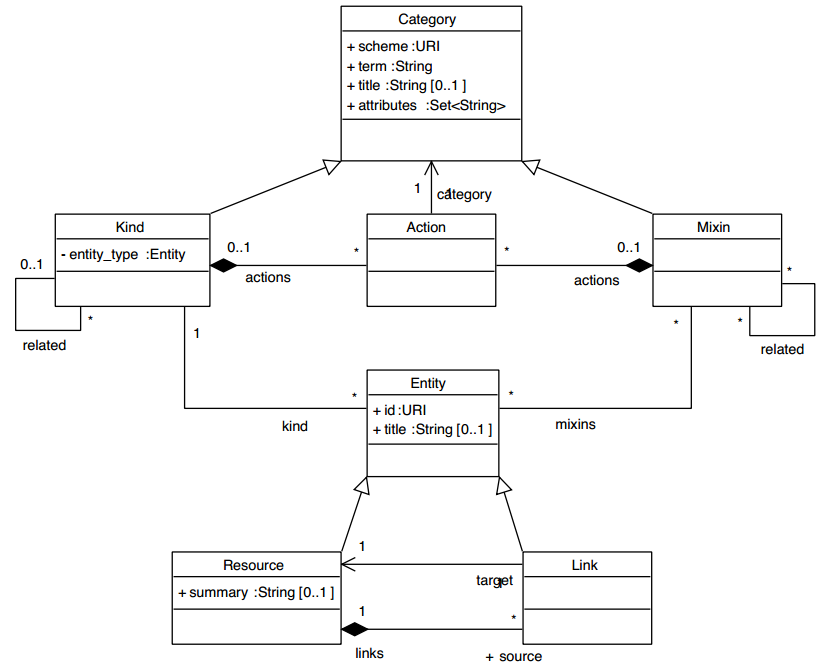
\includegraphics[width=9cm]{images/occi_core_spec}
  \end{center}
\end{frame}

%%%%%%%%%%%%%%%%%%%%%%%%%%%%%%%%%%%%%%%%%%%%%%%%%%%%%%%%%%%%%%%%%%%%%%%%%%%
\begin{frame}
  \frametitle{OCCI}
  \framesubtitle{Infrastructure}

  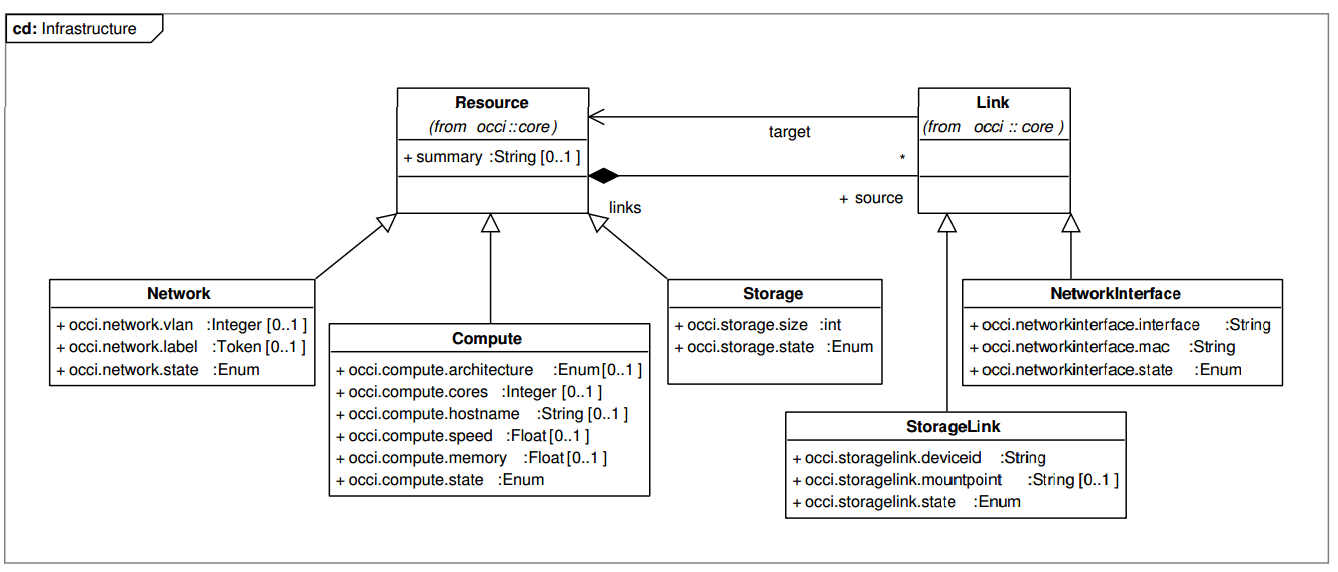
\includegraphics[width=11cm]{images/occi_infra_spec}
\end{frame}

%%%%%%%%%%%%%%%%%%%%%%%%%%%%%%%%%%%%%%%%%%%%%%%%%%%%%%%%%%%%%%%%%%%%%%%%%%%
\begin{frame}
  \frametitle{OCCI}
  \framesubtitle{IaaS Capabilities}

  \begin{columns}
  \begin{column}{0.5\textwidth}
    \begin{enumerate}
        \item Creating VMs
        \item Querying VMs
        \item Destroying VMs
        \item Triggering basic actions on VMs
        \item Creating block storage
        \item Destroying block storage
    \end{enumerate}
  \end{column}

  \begin{column}{0.5\textwidth}
    \begin{enumerate}
    \setcounter{enumi}{6}
        \item Attaching block storage to VMs
        \item Detaching block storage from VMs
        \item Attaching network interfaces to VMs
        \item Detaching network interfaces from VMs
        \item Using contextualization to modify VMs on boot
    \end{enumerate}
  \end{column}
  \end{columns}
\end{frame}

%%%%%%%%%%%%%%%%%%%%%%%%%%%%%%%%%%%%%%%%%%%%%%%%%%%%%%%%%%%%%%%%%%%%%%%%%%%
\begin{frame}[fragile]
  \frametitle{OCCI}
  \framesubtitle{HTTP Rendering}

  \Fontsmaller
  \begin{Sbox}
  \begin{minipage}{\linewidth-2\fboxsep-2\fboxrule-4pt}
  \color{white}
  \begin{verbatim}
POST /compute/ HTTP/1.1

Category: compute;
          scheme="http://.../occi/infrastructure#";
          class="kind"
Category: debian7;
          scheme="http://.../infrastructure/os_tpl#";
          class="mixin"
Category: small;
          scheme="http://.../infrastructure/resource_tpl#";
          class="mixin"
X-OCCI-Attribute: occi.core.title="TestROCCI1"
X-OCCI-Attribute: occi.compute.cores=2
X-OCCI-Attribute: occi.compute.memory=1.7
  \end{verbatim}
  \end{minipage}
  \end{Sbox}
  \fcolorbox{black}{black}{\TheSbox}
\end{frame}

%%%%%%%%%%%%%%%%%%%%%%%%%%%%%%%%%%%%%%%%%%%%%%%%%%%%%%%%%%%%%%%%%%%%%%%%%%%
\begin{frame}
  \frametitle{OCCI}
  \framesubtitle{The rOCCI framework}

  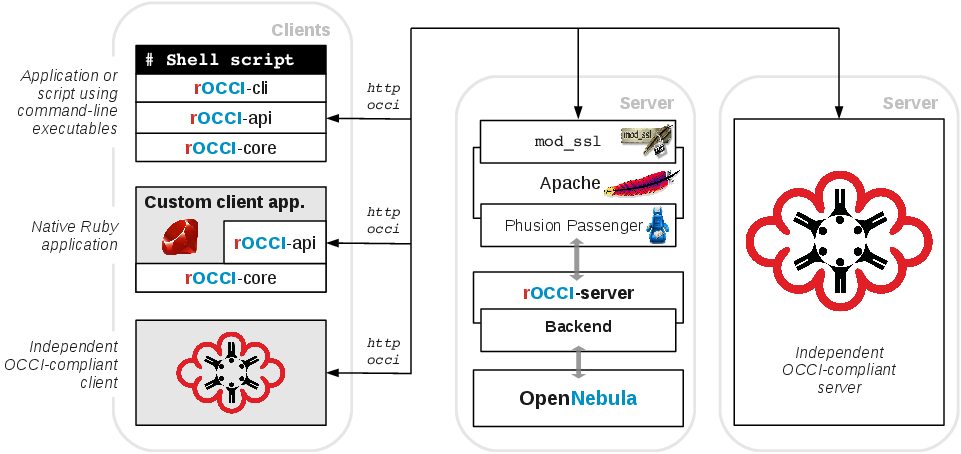
\includegraphics[width=11cm]{images/OCCI_client_servers}
\end{frame}
